\documentclass{article}
\usepackage{listings}
\usepackage{adjustbox}
\usepackage{graphicx}

\title{GGE Manual}
\author{Daniel Johansson}
\date{\today}

\begin{document}
\maketitle
\tableofcontents
\part{GGE in short}
GGE stands for Grid Game Engine (very creative, I know). It is inteded to be used as a game engine for grid based games such as chess or Sid Meier's Civilization. It is not only restricted to turn based games.

The engine itself is written in C++ and depends on SDL2. Games for the engine are written in Guile, a variant of lisp.

There are tools for generating code written in Perl5 though they are not necessary for using the engine.

The following two parts will cover the inner and outer workings of the engine.

The inner working of the engine is not strictly necessary to know when writing a game but it may help understand what happens under the hood. 
This part should be helpful in case of modifying the engine or adding custom game engine modules.

The outer working of the engine is the (Guile) scripting part of it. This is necessary for understanding the process of making a game.
It will also thuroughly describe the example "game" provided.

\part{Inner Workings}

\section{Coding Standards}
Or rather the lack there of. Before anyone gets an aneurysm from reading the code, be aware that this is a project that has been spanning years during which I have developed and changed. What I thought was good coding at the begninning of the
project may not be something I think holds true anymore. 

So why have a whole section on it? 
Aside from personal change there are also two other big contributing factors that I think are important to consider before you burn me at the stake.

First of all there is the fact that my job is to work with ancient legacy Perl code that is almost as old as I am. 
Trying to force coding standards on decade old code where there are none will either take a life time or drive you insane, one does not exlude the other.
Which leads me to the second factor.

In order to not go insane from the jungle that legacy code can be, especially in a language like Perl, I have a Taoist approach.
Rather than forcing what I consider "good" upon the code I adjust and try my best to the standard(s) of the file(s) I'm currently working in.
Rather than pulling my hair because I can't understand what stupid idiot wrote this piece of shit code I take a deep breath I accept that this might just be what was best at the time of writing. 
Adapt to the structures that are there already.
Be like water.
The downside with this approach that sometimes a suboptimal structure remains longer that necessary because the workaround is still easier to work with than to actually properly solve the problem. 
But every once in a while the water will be a tsunami.

The little code standards that exists:
\begin{tabular}{c|c}
	Type & Style \\
	Class & \verb|Class_name| \\
	Variable & \verb|variable_name| \\
	Const & \verb|CONST_NAME| \\
	Function & \verb|function_name| 
\end{tabular}

Data referencing standard:
\begin{enumerate}
	\item Reference (not for storage)
	\item Smart pointer
	\item Pointer (for SDL related data only) (only one object is responsible for freeing the memory pointed to)
\end{enumerate}
I could of course try to make SDL work with smart pointers but using normal pointers works fine. It is not that much of an issue to use. Just keep of track of the pointer. How hard can it be?

\section{The Core}
At the core of GGE is the \verb|Core| object. The \verb|Core| contains \verb|Moduler| for storing and \verb|Runner| running GGE-modules various functions in desired order.
Without the core much of the necessary coordination between objects would not be possible.

\section{Guile - GGE Communication}
Communication between the game, written in Guile, and GGE, written i C++, is done via code found under \verb|script_handling/| and in the center stands the \verb|Scripter| object. 

There are several steps to script communication as illustrated by figure \ref{fig:script_init_example}.
\begin{figure}
	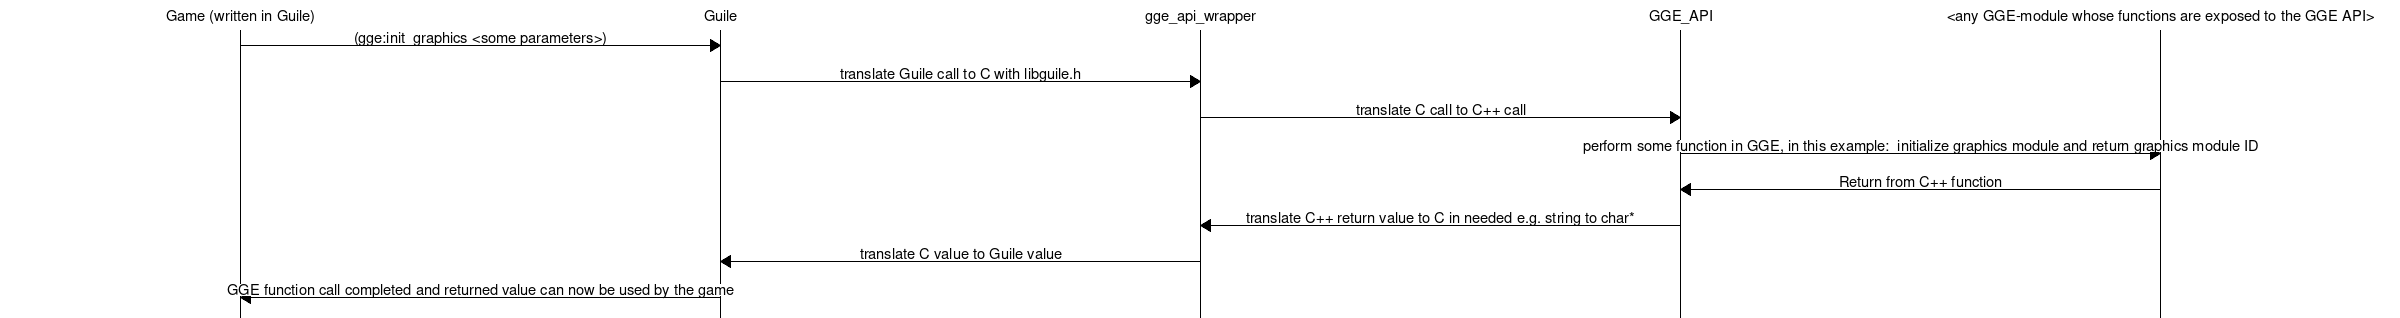
\includegraphics[]{charts/script_communication.png}
	\caption{A call from the game to initialize the graphics module.}
	\label{fig:script_init_example}
\end{figure}

First the \verb|Script| object needs to initialize a script engine object i.e. some class that inherts from the
\verb|Script_engine| class, at the moment of writing only Guile is available, but GGE is open for more.

The script engine object must implement functions necessary for direct communications with the script itself and
whatever is necessary for the script to communicate with a C++ program and the \verb|GGE_API|.
Guile can communicate with C++ via C so a simple C wrapper (C-linked code to be more precise) is necessary.

GGE communicates with the game by having modules exposing their functions to the \verb|GGE_API|. This is done entirely
in C++. Any functionality not exposed to the \verb|GGE_API| can be seen as private member functions of GGE no
available to the game.
Certain core functions are always exposed such as \verb|add_command| and the initialization functions.

The \verb|Scripter| object is not a part of the \verb|Core| object, neither is the \verb|GGE_API| object.

\section{GGE-Modules} \label{inner modules}
GGE performs anything but the bare essentials through GGE-modules, or simply modules. The bare essenatials in this case is memory management and script communication.

A module is really just a class that performs some specfic function. See \ref{standard modules} for list of standard modules.
In order for GGE to be able to use a class as a module it must fullfil certain conditions listed in \ref{reg modules}.
An example of a module is the graphics module. It handles all the graphics related functionality of the engine such as rendering graphics on the screen.

If the game does not initializes any modules GGE can not perform any actions. The \verb|Scripter| object is not a GGE module, it is always initiated.
If the game does not add any commands (see \ref{adding a command}) for initalized modules GGE will not perform any actions with the modules intialized.
You will not even be able to quit the game since no event module that handles input exists, unless it has been written into the game to quit on its own.


In order for the game to make use of a module in the game engine
\begin{enumerate}
	\item Initialize the module to be used.
	\item Add a command for the module if necessary.
	\item When the game is finished initializing and the \verb|Core| object will run the commands in the order given by the script.
\end{enumerate}

\subsection{Standard Modules} \label{standard modules}
Internal module name and class names are only used within the engine. 

\begin{tabular}{|c|c||}
	Internal Module Name & Class Name \\
	\hline
	GRAPHICS & \verb|Graphics| \\
	EVENTS & \verb|Events| \\
	GRID & \verb|Hex_grid| \\
	SCROLLER & \verb|Scroller| \\
	TEXTER & \verb|Texter| \\
	GAME\_LOOP & \verb|Game_loop| \\
\end{tabular}

\subsection{Creating a Module} \label{reg modules}
In order for GGE to see a module it must be registerd in the file \verb|registerd_gge_modules.hpp| in the enum \verb|registered_gge_module|. 
This enum, or rather its integer representation, is returned to the game when the module is initialized.
In order for GGE to use a module it must inherit from the \verb|GGE_module| class. This enables GGE to use polymorphism to handle modules in a generic way, both the \verb|Moduler| and \verb|Runner| use this genericity to handle memory of modules
and calling commands (funcitons of modules) respectively.

Next modules should be initializable via a function in \verb|GGE_initializer|.
These functions should be callable from the \verb|GGE_API| for exposure to the outside.

Now the module can be loaded by the engine. In order to actually make use of the module it is necessary to create
command classes that make use of the module's member functions.

Both intialization functions and command classes one can either be written manually or generated via the Perl scripts in \verb|build_tools/|. See the section \ref{generating code} for how to do so.

\subsection{Command Classes} 
In order for GGE to know what functions to call of what module in which order the command pattern is used.
Each module should have a so-called command class that inherits from the class \verb|Command|.
For example, the \verb|Graphics| module has a \verb|Graphics_command| class.

This command class should contain all the functions one can call from the game. 
This enables GGE to call these functions in the desired order given by the game.

The class \verb|Command| contains
\begin{itemize}
	\item a pointer to the module.
	\item a pointer (that may be null) to the argument.
	\item command.
\end{itemize}
These can be used by its children.

These command classes are used by the \verb|Runner| object by calling each command class' \verb|exeute()| function.
This function will run whichever command it was set to execute when the command class was instantiated.

A command class may contain multiple functions that can be called, but only one can be executed by each command class.
Thus several of each command class my be needed in order to call different functions of the same module.



\subsection{Module Handling}
Once all modules are registered, their functions exposed through the GGE API and have the corresponding 
the command classes they can now be used in the game script. First one needs to specifiy in the game script which modules
to use and in what order the modules functions are to be called. 

Module memory management is handled by the \verb|Moduler| class. Any module can be obtained from the \verb|Moduler| by providing the module's enum.

Module function execution order is handled by the \verb|Runner| class. The \verb|Core| calls the command class functions by calling \verb|Runner.execute()|. Polymorphism is used to call module specific function.

GGE will check to ensure the initialization and call order is correct. 
A failed check will result in an error. 
If the check passed the game will start and GGE will run the modules in the given order.

\subsection{Modules Containing Components}
There are multiple classes making use of the module \verb|Componenter| in order to handle multiple sub structures.
Each class manages the memory of its sub structure. 
These classes can be seen in the table below.
\begin{tabular}{|c|c|}
	Class & sub structure\\
	\verb|Agenter| & \verb|Agent| \\
	\verb|Spriter| & \verb|Sprite| \\
	\verb|Texter| & \verb|Text| \\
\end{tabular}

The class, or file to be more specific \verb|componenter.hpp|, defines the parent structure \verb|Base_component| that is inherited by the sub structures mentioned above. 
The parent structure contains three variables. A boolean that determines if the structure is permanent or not. If it is permanent it will not be checked for removal and the other variables are irrelevant.
A variable that contains the moment of creation and one that contains the life time. 

\subsubsection{Moving an Agent}
This process is a bit wonky. Multiple objects needs to change with the movement of an agent.
First, the Agent structure contains a pointer to the hex it is standing on and a pointer to its sprite.
Second, the tile the agent is placed on also has a pointer to the agents standing on it. 

When an agent is to be moved the following steps must take place.
\begin{itemize}
	\item The new tile must point to the agent.
	\item The old tile must not point to the agent anymore.
	\item The agent must point to the new tile it is moving to.
	\item The agent's sprite must be repositioned to the new tile so that the move can be seen graphically.
\end{itemize}

There is an internal class, \verb|Move_agent|, within the Agent class that handles these steps. 

\subsection{Grid and Tile}


\section{Generating Code} \label{generating code}
Perl5 is used to generate a bunch of code. This is not necessary in order to run the engine. 
While not strictly necessary to use when modding the engine there are unfortunately some places of the code that
require repetitive coding which can be skipped with the scripts in \verb|build_tools/|.
Simply run all scripts ending in \verb|.pl| and all necessary code will be generated. 
The table below describes the different scripts and their functions.

\begin{adjustbox}{width=\paperwidth}
\begin{tabular}{|c|c|l|}
	Script Name & Writes to & Description \\
	\verb|expand_gge_module.pl| & \verb|gge_module.hpp| & Generates cases for stringifying a modules name \\
	\verb|expand_modules.pl| & \verb|moduler.hpp| and \verb|moduler.cpp| & 
	Generates getters and setters for modules \\
	\verb|expand_modules.pl| & \verb|moduler.hpp| and \verb|moduler.cpp| & 
	Generates getters and setters for modules in the Moduler object as well as necessary includes \\
	\verb|generate_commands.pl| & \verb|commands/<specific_command>.hpp| & 
	Generates classes for specific commands\\
	\verb|generate_get_gge_modules.pl| & \verb|generated_get_gge_modules| & 
	DEPRECATED \\
	\verb|generate_gge_api_defaults.pl| & \verb|gge_api_defaults.generated| & 
	Generates template code for exposing functions in the \verb|GGE_API| to Guile \\
\end{tabular}
\end{adjustbox}

\textit{
	Note: the Perl scripts to not check for errors nor always generate nicely formated code.
	Make sure your code is correct or finding erros will be a hassle.
}

\part{Outer Workings}

\section{Guile}
The games for GGE are written in Guile is an implementation of Scheme, which is a dialect of Lisp. 

The game should be all contained in one directory. This directory should be used as a parameter to GGE.

GGE will be looking for a two important files.

First \verb|init.scm|. This is where module initialization of modules and addition of commands should take place.

Second \verb|game.scm| where a function called \verb|game_loop| should exist. In this function game logic should reside.

\section{Modules}

If you want to use a non-standard module please read through section \ref{inner modules}.

\subsection{Initializing a Module}
Modules are initialized through the \verb|gge_api| functions found in the \verb|gge| module.
The function will return an integer that represents the ID (enum) of the module used inside GGE. This can be useful for when adding commands.
Example: \verb|(init_graphics "GGE Test" 640 480))|

\subsection{Adding a Command} \label{adding a command}
Once modules have been initiated commands can be added to the module through the \verb|gge_api| function \verb|add_command|
Example: \verb|(add_command game_loop)|

GGE will check to ensure the initialization and call order is correct. 
A failed check will result in an error and not continue running the script.


\end{document}
